\documentclass[a4paper,12pt]{article}


\usepackage{natbib}

\usepackage{float}

\usepackage[utf8]{inputenc}

%Rajoute des régles de typo
\usepackage[french]{babel}
%Change l'accent
\usepackage[T1]{fontenc}
\usepackage{hyperref}
\usepackage{enumitem}
\usepackage{amsmath,amssymb}

\usepackage{color}

\usepackage{graphicx,xcolor}
\usepackage{subcaption}
\usepackage{geometry}
\geometry{left=1.5cm, right=1.5cm, bottom=2cm, }
\newcommand{\rmq}[1]{\textcolor{red}{#1}}

%Pour les définitions
\usepackage{amsthm}
\newtheorem{mydef}{Definition}

\begin{document}

	\newcommand{\HRule}{\rule{\linewidth}{0.5mm}}

	\begin{titlepage}

		\center

		\textsc{\LARGE Sorbonne université}\\[1.5cm] % Name of your university/college

        \begin{minipage}{0.4\textwidth}
		\begin{flushleft} \large
		\end{flushleft}
		\end{minipage}




		\textsc{\huge \bfseries Rapport de ARF}\\[.5cm]

		\HRule \\[0.4cm]
		{ \huge \bfseries TME 1 - 6 }\\[0.4cm]
		\HRule \\[4cm]

		{ \huge \textsc{Samu Tamminen} }

		\vfill
		Année 2017-2018
	\end{titlepage}



\newpage
\tableofcontents
\newpage

\section{TME 1 : Arbres de décision, sélection de modèles}

\subsection{Q1.3 Interpretation de l'entropie}
Calculer également la différence entre l’entropie et l’entropie conditionnelle pour chaque attribut.
A quoi correspond une valeur de 0 ? une valeur de 1 ? Quel est le meilleur attribut pour la première partition?
\\
Quand la différence entre l'entropie et l'entropie conditionnelle est 0 quand la partition n'est pas du tout bon et un,
quand la partition est le meilleur possible.

\subsection{Q1.4 - 6 La profondeur d'arbre }

En augmentant la profondeur maximale d'arbre, on obtient meilleur score.
Mais ces scores ne sont pas un indicateur fiable, si nous ne faisons pas différence entre les données training et test.

\subsection{Q1.7 -  Sur et sous apprentissage }

Le partition 0.8 / 0.2 dans ~\autoref{fig:tme1_scores} (c) semble d'etre le plus robust pour test et training.
La difference difference entre le score dans aprentissage et test est le plus petit parmis (a),(b) et (c).

Quand il y a que peu d'examples d'apprentissage, l'erreur est plus éleve dans le test.
Par contre quand on a beacoup des d'examples d'aprentissage, l'erreur dans le test est moins d'élevé.

Avec validation croisée on obtient un score plus fiable et stable.
Dans la figure \autoref{fig:tme1_scores} (d) nous pouvons constater, comment le score augmente au début avec la profondeur maximale, mais à la fin il tombe.
Ça c'est à cause de sous et sur apprentissage.
Au début, on généralise beaucoup avec un arbre peu profond (sous apprentissage).
Quand la profondeur se monte sur cinq,
nous commençons à apprendre les données d'apprentissage à la façon trop détaillée et le score sur le test se tombe (sur aprentissage).
La profondeur maximale 4 semble optimal.

\begin{figure}
\caption{Score d'arbre de decision en faisant varier le profondeur}
\label{fig:tme1_scores}
\begin{subfigure}{.5\textwidth}
	\centering
	\label{fig:partition_2_8}
	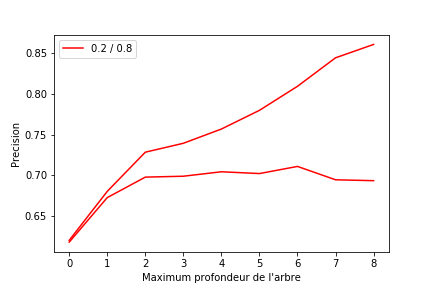
\includegraphics[width=0.4\linewidth]{images/tme1/partition_2_8.png}
	\caption{Donnée aprentissage et test : 0.2 / 0.8}
\end{subfigure}%
\begin{subfigure}{.5\textwidth}
  \centering
	\label{fig:partition_5_5}
	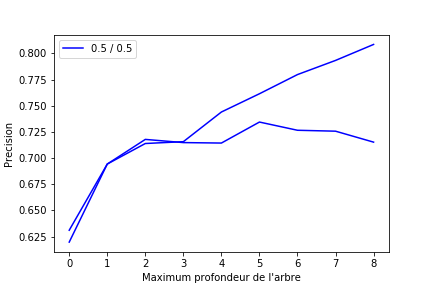
\includegraphics[width=0.4\linewidth]{images/tme1/partition_5_5.png}
	\caption{Donnée aprentissage et test : 0.5 / 0.5}
\end{subfigure}
\begin{subfigure}{.5\textwidth}
  \centering
	\label{fig:partition_8_2}
	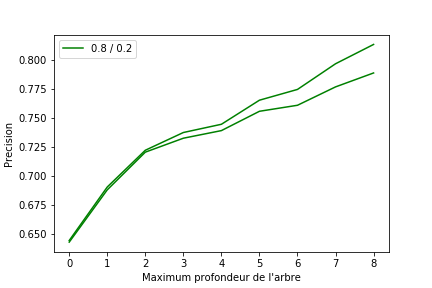
\includegraphics[width=0.4\linewidth]{images/tme1/partition_8_2.png}
	\caption{Donnée aprentissage et test : 0.8 / 0.2}
\end{subfigure}
\begin{subfigure}{.5\textwidth}
  \centering
	\label{fig:partition_vc}
	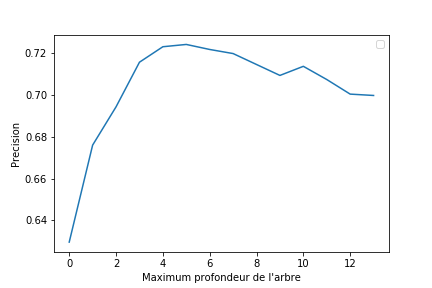
\includegraphics[width=0.4\linewidth]{images/tme1/partition_vc.png}
	\caption{Validation croisee}
\end{subfigure}
\end{figure}

\section{TME 2 : Estimation de densité}

\section{TME 3 : Descente de gradient}

\section{TME 4 et 5 : Perceptron}

\section{TME 5 : Support Vector Machine}


\subsection{Pistes de recherche}

\end{document}
